% ==============================================================
%  Chapter 3 -- Implementation
% ==============================================================

\chapter{Implementation}
\label{ch:implementation}

This chapter describes the implementation used to estimate the parameter vector $\boldsymbol{\Theta}$ of a regular
Influence Diagram from a partial expert rule base $\mathcal{R}$.
The system is built on top of two external components: the
\textsc{SMILE} reasoning engine and its \texttt{pysmile} Python library,
which provide the \texttt{.xdsl} parser and the Shachter evaluation
algorithm~\cite{shachter1986evaluating,genie}; and
\textsc{EDAspy}, the open-source library of Soloviev et al.~\cite{soloviev2024edaspy} that implements the EDA variants
discussed in Chapter~\ref{ch:framework}. Around these dependencies the
system is organised in four functional layers:

\begin{enumerate}
    \item \textbf{Model loading and structural extraction.}
          The \texttt{.xdsl} file is parsed into an internal node
          dictionary that holds the graph structure and a
          \texttt{NumPy} reference to every numerical table.
    \item \textbf{Rule-base parsing.}
          The expert rule base is read from a CSV file and translated
          into a list of $(\mathbf{evidence},\, D_{i_l},\, a^{(l)})$
          triples.
    \item \textbf{Fitness evaluation.}
          For each candidate parameter vector, the Shachter engine is
          invoked once per rule and the losses are aggregated
          into the score the EDA tries to minimise.
    \item \textbf{EDA-based optimisation.}
          The continuous EDA variants of \textsc{EDAspy} drive
          the search over an encoded parameter vector
          $\boldsymbol{\phi}$.
\end{enumerate}



% ==============================================================
\section{Model structural extraction and rule parsing}
% ==============================================================

The diagram is read once with the \texttt{pysmile} library, which exposes every
node, its parents and its CPT. The pipeline keeps a reference to each table so that a candidate solution can be written back
in place from the parameter vector and the diagram re-evaluated without rebuilding the network every time; the evaluation is by far the most expensive operation, so it
is repeated as little as possible.

The expert rules are synthetically created by evaluating the network multiple times, each with a different possible combination of events. Then they are stored in a CSV file with one rule per row. Each row
records the observed state of the relevant variables and the action the
expert considers optimal for the target decision; a sign convention
distinguishes the observed variables from the target decision and marks
the columns that play no role in that rule (any node that is not a parent of the decision node). Only rows that actually name
a target decision are kept. The result is a list of
\emph{(evidence, decision, expected action)} triples that the scoring
step will check one by one.

\subsection{A real example: the \emph{bypass} influence diagram}
\label{sec:bypass-example}

Throughout the rest of the chapter we ground the description on the
\emph{bypass} ID, a small clinical model that we adopt as the
illustrative network of this work. It contains six chance nodes
(\textsf{HeartDisease}, \textsf{Angiogram}, \textsf{Pain},
\textsf{EarlyResults}, \textsf{LifeQ}, \textsf{Economicalc}), two
decision nodes (\textsf{HeartSurgery}, \textsf{HeartPharma}) and a
single utility node. Its qualitative structure is shown in
Figure~\ref{fig:bypass-id}.

\begin{figure}[H]
    \centering
    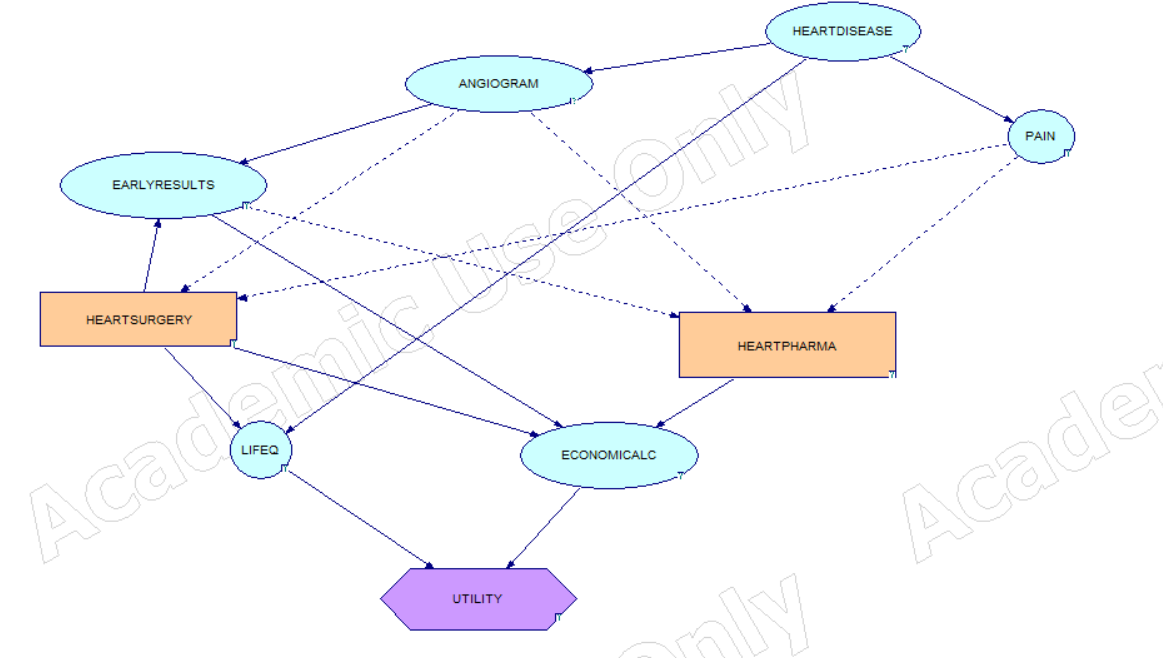
\includegraphics[width=0.85\linewidth]{figures/bypass.png}
    \caption{Influence diagram of the \emph{bypass} model. Chance
    nodes are ellipses, decision nodes rectangles and the utility
    node a hexagon; dashed arcs are informational, solid arcs are
    probabilistic or functional.}
    \label{fig:bypass-id}
\end{figure}

To make explicit what kind of objects the algorithm manipulates, we
extract one CPT directly from the model. The chance node
\textsf{Angiogram} (test result) depends only on \textsf{HeartDisease}
(the true underlying condition), and its table is reproduced in
Table~\ref{tab:bypass-cpt}: it amounts to the standard
sensitivity/specificity of the test.

\begin{table}[H]
\centering\small
\begin{tabular}{l|cc}
\hline
$P(\textsf{Angiogram} \mid \textsf{HeartDisease})$
              & \textsc{negative} & \textsc{positive}\\
\hline
$\textsf{HeartDisease} = \textsc{absent}$  & 0.95 & 0.05\\
$\textsf{HeartDisease} = \textsc{present}$ & 0.14 & 0.86\\
\hline
\end{tabular}
\caption{Real CPT extracted from the bypass model: angiogram
sensitivity and specificity given the true heart-disease status.
This is one of the rows of the parameter vector $\boldsymbol{\Theta}$
that the EDA must recover when it is unknown.}
\label{tab:bypass-cpt}
\end{table}

The rule base is a CSV file with one row per rule and one column per
node of the diagram. Sign convention: a positive integer
$+v$ encodes that the corresponding chance node is observed in its
$(v{-}1)$-th state; a negative integer $-v$ identifies the target
decision node and the action $(\lvert v\rvert{-}1)$ the expert prescribes
for it; the value $0$ marks the node as irrelevant for that
particular rule (in practice, it is a node that is not an
informational parent of the target decision). For the bypass model
the eight columns are
\textsf{ANGIOGRAM, EARLYRESULTS, ECONOMICALC, HEARTDISEASE, LIFEQ,
PAIN, HEARTPHARMA, HEARTSURGERY},
and the very first row of \texttt{reglas\_generadas.csv} reads
\begin{center}
\texttt{1, 1, 0, 0, 0, 1, -1, 0}
\end{center}
which, decoded with the state mappings of the model, becomes the
explicit rule
\begin{quote}
\emph{If \textsf{Angiogram}~$=$~\textsc{negative} \;and\;
\textsf{EarlyResults}~$=$~\textsc{CoRem} \;and\;
\textsf{Pain}~$=$~\textsc{absent},
\quad then \;\textsf{HeartPharma}~$=$~\textsc{no}.}
\end{quote}
Evaluating this rule means: write the decoded $\boldsymbol{\Theta}$
into the model, enter the three observed states as evidence, run
Shachter on \textsf{HeartPharma} and check that its optimal action is
\textsc{no}. The fitness of the candidate is the aggregated per-rule
loss over the whole \texttt{reglas\_generadas.csv}, computed in the
next section.

% ==============================================================
\section{Encoding and decoding the parameters}
% ==============================================================

The EDA searches over plain real vectors, but the parameters of an ID
are constrained: every CPT row must be a probability distribution and
the utilities must stay on a bounded scale. The encoding keeps the two
worlds apart. The optimiser works on a \emph{raw} vector
$\boldsymbol{\phi}$ whose entries it samples freely within symmetric
bounds — in our runs $[-5,5]$ for the CPT entries and $[-10,10]$ for the
utilities — and a \emph{decoder} turns that raw vector into a valid
model. As mentioned earlier, a fixed node ordering encoded in a dictionary tells the decoder which slice of
$\boldsymbol{\phi}$ belongs to each table.

Decoding is where the constraints are enforced, through two squashing
functions applied row by row:

\begin{itemize}
  \item \textbf{Chance nodes --- softmax with $\varepsilon$-floor.}
        Each CPT row is first softened by the softmax,
        $\tilde{\theta}_j = \operatorname{softmax}(\boldsymbol{\phi}_{\text{row}}/T_c)_j$,
        which already returns non-negative values that sum to one. To
        prevent any entry from being exactly $0$ or $1$ (degenerate
        CPTs that make subsequent evaluations brittle and forbid
        recovery from a wrong commitment), we additionally floor each
        entry at a small constant $\varepsilon$ and renormalise the
        row:
        \[
            \hat{\theta}_j = \frac{\max(\varepsilon,\,\tilde{\theta}_j)}
                                  {\sum_k \max(\varepsilon,\,\tilde{\theta}_k)}.
        \]
        With $\varepsilon = 10^{-3}$ this guarantees
        $\hat{\theta}_j \in [\varepsilon',\, 1-\varepsilon']$ for some
        small $\varepsilon'>0$ depending on $\varepsilon$ and the row
        cardinality, while preserving the simplex constraint.
  \item \textbf{Utility node --- sigmoid.} Each free utility entry is the
        sigmoid of its raw value, rescaled to the chosen range
        $[u_{\min},u_{\max}]$ (here $[0,10]$):
        $\hat{u} = \sigma(\phi/T_u)\,(u_{\max}-u_{\min}) + u_{\min}$. Two
        entries are then pinned to the best and worst outcomes declared
        by the expert. Because the raw values are clipped to a bounded
        box before squashing, the sigmoid never saturates fully and the
        decoded utilities stay strictly inside the interior of the
        $[u_{\min},u_{\max}]$ range, i.e.\ they never reach exactly
        $u_{\min}$ nor $u_{\max}$ except at the two pinned entries.
\end{itemize}

\begin{proposition}[Validity of the decoded model]
\label{prop:valid-cpt}
For every raw vector $\boldsymbol{\phi}$ the decoded tables form a valid
parameterisation: softmax guarantees that each CPT row is non-negative
and sums to one, and the rescaled sigmoid keeps every utility inside
$[u_{\min},u_{\max}]$. The Shachter engine can therefore be evaluated
unconditionally, with no need to reject or repair samples.
\end{proposition}

However, these two squashing functions are not innocuous; their consequences are
worth explaining in detail:

\begin{itemize}
  \item \textbf{No repair step.} Because softmax and sigmoid land on the
        feasible set by construction, the EDA can explore an
        \emph{unconstrained} real space while the decoded model will remain always
        valid (there will never be a sample to clip or discard).
        This is what makes the row-wise validity of
        Proposition~\ref{prop:valid-cpt} come for free.
  \item \textbf{Temperatures control sharpness.} The temperatures
        $T_c, T_u$ rescale the raw values before squashing. A low $T_c$
        pushes a CPT row towards a near-deterministic distribution (all
        the mass on one state); a high $T_c$ flattens it towards the
        uniform. The sigmoid behaves analogously for the utilities,
        sharpening or softening the contrast between outcomes. In summary, the temperature controls the entropy of the parameter vector and, as we will see later, introduces a trade-off effect for certain fitness functions.
        
  \item \textbf{Monotonicity and saturation of the utility.} The sigmoid
        is monotone, so the \emph{ordering} of the raw utility values
        is preserved in the decoded utilities (which is all that
        matters, since the optimal policy depends only on that ordering).
        Its saturation, however, means that most of the sensitivity is
        concentrated near the midpoint of the range: extreme raw values
        barely move the decoded utility, so the optimiser has fine
        control over close calls and coarse control at the extremes.
\end{itemize}

Finally, the two pinned utility entries are not cosmetic. Because the
optimal policy depends only on the ordering of the utilities, $u$ is
identifiable only up to a positive affine transformation; fixing the
best and worst outcomes removes that ambiguity and stops the EDA from
drifting along a direction that does not change the policy. 

% ==============================================================
\section{Scoring a candidate}
% ==============================================================

A candidate is scored by how well the policy it induces reproduces the
expert rules. This is the mean per-rule loss
$\mathcal{L}(\boldsymbol{\Theta})$ of
Definition~\ref{def:fitness}, which \textsc{EDAspy} minimises directly.
A central point is that this loss is \emph{not unique}: the per-rule
term $\ell$ is a configurable choice, and the implementation exposes the
whole family introduced in Chapter~\ref{ch:framework} — the $0$--$1$
\textsc{binary} loss, \textsc{regret}, \textsc{margin}, \textsc{softmax}
and \textsc{entropy} — whose effect on convergence and final accuracy is
compared experimentally in Chapter~4. The simplest member is the
$0$--$1$ loss, whose mean is just the fraction of rules the model gets
wrong:

\begin{definition}[Rule-accuracy loss]
\label{def:cost}
With the $0$--$1$ per-rule loss, the objective reduces to
\[
   \mathcal{L}\bigl(\boldsymbol{\Theta}(\boldsymbol{\phi})\bigr) =
   \frac{1}{|\mathcal{R}|}
   \sum_{(\mathbf{x}^{(l)}, D_{i_l}, a^{(l)})\in\mathcal{R}}
   \mathbb{1}\!\left[\delta^{*}_{i_l}\!\left(\boldsymbol{\Theta}
   (\boldsymbol{\phi}),\mathbf{x}^{(l)}\right) \neq a^{(l)}\right],
\]
where $\boldsymbol{\Theta}(\boldsymbol{\phi})$ is the decoded vector and
$\delta^{*}_{i_l}$ is the action the Shachter engine returns under the
evidence $\mathbf{x}^{(l)}$. The smoother variants replace the
indicator by the corresponding $\ell$ of
Chapter~\ref{ch:framework}, exposing more gradient-like information to
the search.
\end{definition}

Whatever the loss, evaluating one candidate means decoding it into the
tables and, for each rule, entering its evidence, running the diagram and
inspecting the recommended action.

% ==============================================================
\section{The optimiser}
% ==============================================================

\textsc{EDAspy}~\cite{soloviev2024edaspy} is the reference open-source
EDA library of the UPM CIG group; it implements the univariate and
multivariate variants reviewed in Chapter~\ref{ch:framework} behind a
common interface. The pipeline plugs into this library and exposes
four of its continuous variants:
\begin{itemize}
  \item \texttt{UMDAc} — independent Gaussian marginals (no
        cross-parameter dependencies).
  \item \texttt{EMNA} — multivariate Gaussian with full covariance
        (all pairwise dependencies, no structure).
  \item \texttt{EGNA} — Gaussian Bayesian network with structure
        learnt every generation (a sparse multivariate model).
  \item \texttt{KEDA (univariate)} — kernel-density marginals (no
        Gaussian assumption per dimension).
\end{itemize}
Together they form a spectrum from fully factorised to fully
multivariate, and from parametric to non-parametric. Which one is
preferable for the parameter-recovery problem is not obvious a priori
(full covariance is more expressive but more costly to estimate). We therefore leave the
choice to the empirical comparison of Chapter~4. Richer variants such
as SPEDA, also implemented in \textsc{EDAspy}, are left to the
perspectives chapter.

The run is governed by the few hyperparameters of
Table~\ref{tab:hyperparams}. The search stops early when the best cost
does not improve for $T_{\text{dead}}$ consecutive generations, which
avoids wasting time once the population has converged.

\begin{table}[h]
\centering\small
\begin{tabular}{lll}
\hline
\textbf{Hyperparameter} & \textbf{Symbol} & \textbf{Role}\\
\hline
\texttt{optimizer\_type} & --- & UMDA, EMNA, EGNA or KEDA\\
\texttt{size\_gen}       & $N$ & Individuals per generation\\
\texttt{max\_iter}       & $T$ & Maximum number of generations\\
\texttt{dead\_iter}      & $T_{\text{dead}}$ & Early-stopping patience\\
\texttt{alpha}           & $\mu$ & Truncation selection ratio\\
\texttt{elite\_factor}   & $\mu_{el}$ & Fraction of best individuals preserved\\
\hline
\end{tabular}
\caption{Main hyperparameters used in this work.}
\label{tab:hyperparams}
\end{table}

The first population is drawn \emph{uniformly} within the symmetric raw
bounds. This choice is deliberate. Because the bounds are centred at
zero and both squashing functions are symmetric, a raw value of
zero decodes to a uniform CPT row and to the mid-range utility. The
search therefore starts \emph{unbiased}, with no built-in preference for
any state of a chance node or any action of a decision. Uniform sampling
also scatters the initial individuals across the whole raw space rather
than around a single guess, so the EDA explores broadly before its model
contracts — which matters on the multimodal, degenerate landscape of
this problem, where many parameter vectors reproduce the same rules and
an early commitment to one region would be premature.

A natural extension, supported by \textsc{EDAspy} and discussed
in the perspectives chapter, replaces this uninformed start: an
LLM-generated warm start~\cite{nafar2025llm4bn}.



